% Compile with: latexmk -pdf lean-search-bench.tex   (pdfLaTeX + BibTeX)
% Format follows the Lean Census and Fuse papers.
% figures/forms.pdf and scores.json are produced by figures.py.
\documentclass{article}
\PassOptionsToPackage{numbers,compress}{natbib}
\usepackage[preprint]{neurips_2025}
\usepackage[utf8]{inputenc}
\usepackage[T1]{fontenc}
\usepackage{microtype}
\usepackage{amsmath,amssymb}
\usepackage{booktabs}
\usepackage{tabularx}
\usepackage{enumitem}
\usepackage{xcolor}
\usepackage{colortbl}
\usepackage{graphicx}
\usepackage{float}

% Numina palette (shared with the Fuse and Lean Census papers).
\definecolor{nAccent}{HTML}{BB480B}
\definecolor{nInk}{HTML}{222222}
\definecolor{nMuted}{HTML}{6B5B4A}
\definecolor{nBorder}{HTML}{D6CFC0}
\definecolor{nBorderLight}{HTML}{EDE6DA}

\usepackage[font=small,labelfont={bf,color=nAccent},labelsep=period]{caption}
\captionsetup[table]{skip=8pt}
\usepackage[colorlinks=true,linkcolor=nAccent,citecolor=nAccent,urlcolor=nAccent]{hyperref}
\arrayrulecolor{nBorder}

\newcommand{\thead}[1]{\textbf{#1}}
\newcommand{\rowrule}{\arrayrulecolor{nBorderLight}\specialrule{0.4pt}{3pt}{3pt}\arrayrulecolor{nBorder}}
\renewcommand{\bottomfraction}{0.6}
\renewcommand{\textfraction}{0.1}
\renewcommand{\topfraction}{0.9}
\renewcommand{\floatpagefraction}{0.8}
\setlist{itemsep=2pt,topsep=3pt}
\raggedbottom
\newcommand{\code}[1]{\texttt{\small #1}}
% The name of the benchmark, in one place so that it can be changed.
\newcommand{\bench}{DeclSearch}
\newcommand{\todo}[1]{\textcolor{red}{[TODO: #1]}}

\title{\bench: A Benchmark for Lean 4 Declaration Search}
\author{%
  Justin Asher$^{1}$\hspace{1.4em}Pietro Pellegrino$^{1,2}$ \\[1.2ex]
  \small\normalfont $^{1}$Project Numina \\[0.3ex]
  \small\normalfont $^{2}$University of Naples Federico II \\[0.8ex]
  \small\normalfont \texttt{justin@projectnumina.ai}\hspace{1.4em}\texttt{pietro@projectnumina.ai}
}

\begin{document}
\maketitle

\begin{abstract}
We present \bench, a benchmark for search engines over Lean 4 declarations. It
has 3,200 queries about Mathlib in four equally weighted buckets: names and
keywords, natural language, formal statements and proof states, and questions
derived from Lean Zulip threads. Every answer is a declaration that all
current engines index, and answers were completed by grading the results of
four engines blind. We compare it with existing benchmarks and report scores
for four hosted engines and a BM25 baseline. This is version 1, and we expect
the benchmark to change. Queries, labels, engine results, and code are at
\url{https://github.com/lean-explore/lean-explore-bench}.
\end{abstract}

%=====================================================================
\section{Introduction}

Several engines search Lean~\cite{moura2021lean4} declarations:
Loogle~\cite{breitner2023loogle} by name and pattern, and
LeanSearch~\cite{gao2024leansearch,gao2026leansearchv2},
LeanExplore~\cite{asher2025leanexplore}, and Lean
Finder~\cite{lu2025leanfinder} by meaning. Each was evaluated by its authors
on their own queries, so their published numbers cannot be compared. We need a
fixed benchmark to compare engines and to measure changes to our own.

\bench\ is that benchmark. It differs from existing ones
(Section~\ref{sec:existing}) in three ways.
\begin{itemize}
\item \textbf{Query forms.} It covers the forms that searches take, from a
bare name to a proof state, and includes questions from real discussions.
\item \textbf{Answers.} A query can have several answers. We graded what four
engines returned and added every result that answers the query.
\item \textbf{Fairness.} Every answer is a Mathlib~\cite{mathlib2019}
declaration that all engines index, and the score weights four kinds of search
equally and not by the traffic of any engine.
\end{itemize}

This paper describes version 1. Section~\ref{sec:future} lists what we plan to
change.

%=====================================================================
\section{Existing benchmarks}
\label{sec:existing}

Table~\ref{tab:existing} lists the query sets that Lean search engines have
been evaluated on.

\begin{table}[t]
\centering\small
\caption{Benchmarks for Lean declaration search. Lean Finder has five test
sets of 1,000 to 2,224 queries each.}
\label{tab:existing}
\begin{tabularx}{\linewidth}{@{}lrXl@{}}
\toprule
\thead{Benchmark} & \thead{Queries} & \thead{Query styles} & \thead{Answers per query} \\
\midrule
LeanSearch~\cite{gao2024leansearch} & 50 & description, \LaTeX, theorem name, Lean term & several, graded \\
\rowrule
MathlibQR~\cite{gao2026leansearchv2} & 946 & six styles written by experts for 200 declarations & one \\
\rowrule
Lean Finder~\cite{lu2025leanfinder} & 7,448 & informal statements, synthetic user queries, perturbed formal statements, proof states & one, exact match \\
\rowrule
LeanExplore~\cite{asher2025leanexplore} & 300 & short topical queries & none \\
\rowrule
\bench\ (ours) & 3,200 & eight forms in four buckets, one from real questions & 1.6 on average, graded \\
\bottomrule
\end{tabularx}
\end{table}

\paragraph{Single answers.} MathlibQR and the Lean Finder sets label one
declaration per query, and Lean Finder counts a hit only on an exact match.
Mathlib often has several declarations that answer a query, and an engine that
returns another one is marked wrong. On \bench, adding the answers found
by pooling raised the score of the three semantic engines by 5 to 8 points
(Section~\ref{sec:results}).

\paragraph{Query styles.} The LeanSearch set has 50 queries. The LeanExplore
set has no labelled answers, and a language model ranked the engines instead.
MathlibQR is written by experts and balanced over Mathlib, but it has no proof
states and no queries from real use. The Lean Finder sets cover proof states
but are synthetic and were built by the authors of that engine.

\paragraph{Coverage.} Engines index Mathlib at different dates, and an engine
cannot return a declaration it has not indexed. MathlibQR handles this with a
subset of 810 queries whose answers every compared system holds. We apply the
same rule to the whole benchmark.

Premise selection benchmarks~\cite{yang2023leandojo,tao2025premise} ask for
the lemmas that a proof uses, and MIRB~\cite{ju2025mirb} collects mathematical
retrieval tasks for embedding models. Both evaluate models on a fixed corpus,
not search engines as deployed.

%=====================================================================
\section{The benchmark}
\label{sec:benchmark}

\subsection{Queries}

Every query has one of eight forms, decided by its surface alone
(Table~\ref{tab:forms}). We took the forms and their typical lengths from an
analysis of LeanExplore's search traffic. No user query is in the benchmark.

\begin{table}[t]
\centering\small
\caption{The eight forms of a query, with an example of each from the
benchmark.}
\label{tab:forms}
\begin{tabularx}{\linewidth}{@{}llX@{}}
\toprule
\thead{Form} & \thead{Definition} & \thead{Example} \\
\midrule
\code{name} & One Lean name & \code{Polynomial.Separable.of\_mul\_right} \\
\rowrule
\code{names} & Several Lean names & \code{IsOpen Set.singleton pure\_le\_nhds} \\
\rowrule
\code{names+keywords} & Names and other words & \code{Finsupp.prod} embedding domain support \\
\rowrule
\code{keywords} & Words, no function words & combine family affine maps into product space \\
\rowrule
\code{prose} & Natural language & tail of interleaving two infinite streams \\
\rowrule
\code{prose+names} & Natural language with names & prenex conversion of a \code{BoundedFormula} is prenex \\
\rowrule
\code{formal} & A Lean statement or pattern & \code{ManyOneEquiv u v $\to$ (ManyOneEquiv u w $\leftrightarrow$ ManyOneEquiv v w)} \\
\rowrule
\code{goal} & A proof state & \code{$\vdash$ WithBot.succ x = $\bot$ $\leftrightarrow$ x = $\bot$} \\
\bottomrule
\end{tabularx}
\end{table}

The forms are grouped into four buckets of 800 queries
(Table~\ref{tab:buckets}). \textbf{The benchmark score is the plain mean of
the four bucket scores.} We do not weight by traffic. People send an engine
what it handles well, so the traffic of any one engine favours that engine.

\begin{table}[t]
\centering\small
\caption{The four buckets.}
\label{tab:buckets}
\begin{tabular}{@{}lrl@{}}
\toprule
\thead{Bucket} & \thead{Queries} & \thead{Made of} \\
\midrule
Names and keywords & 800 & 160 \code{name}, 80 \code{names}, 240 \code{names+keywords}, 320 \code{keywords} \\
\rowrule
Natural language & 800 & 480 \code{prose}, 320 \code{prose+names} \\
\rowrule
Formal & 800 & 480 \code{formal}, 320 \code{goal} \\
\rowrule
Real questions & 800 & queries derived from Lean Zulip threads \\
\bottomrule
\end{tabular}
\end{table}

\subsection{Answers}

Every answer is a Mathlib declaration with the same name and module in a
January 2026 snapshot, which 88\% of the declarations in our July 2026 corpus
have. Without this rule the benchmark measures what an engine indexes. In an
earlier build, on queries about declarations added after January 2026,
LeanSearch and Lean Finder found no answers at all, against 93\% and 95\% on
older declarations.

Answers are graded from 1 to 3. Grade 3 is a direct answer and grade 2 is
useful after a clear adaptation. Both count as a hit.

\subsection{Construction}

\paragraph{Written queries.} The first three buckets are written from a
target declaration drawn at random from Mathlib. A language model sees the
target and writes a query of a given form and length. \code{name} queries are
made by rule, as the full name or a variant with a missing namespace, a typing
error, or another small change. A query is kept if it has the form asked for, does not
leak the target's name, and a judge from another model family
(\code{openai/gpt-6.1-terra}) grades the target 3 and finds the query
specific to it. Claude Opus wrote 1,294 of the 2,400 written queries. It
reviewed another 946 written by Claude Sonnet 5.5, and rewrote 322 of them.

\paragraph{Real questions.} The fourth bucket comes from Lean Zulip threads in
which someone asks for a result and a reply names a declaration. A language
model writes the search that the asker might have typed, using nothing from
the replies. The declarations named in the replies are proposed answers, and
the query is kept if the judge grades at least one of them 2 or 3. The
benchmark contains no text of any post: a query that repeats more than five
consecutive words of a message is rejected. \todo{515 queries are not yet
checked against their thread.}

\paragraph{Pooled answers.} A written query starts with one answer. To find
the others we pooled the first ten results of four engines for each
query~\cite{sparckjones1975pooling,voorhees2005trec}, cut each list at its
first labelled answer, and removed candidates that the rule above excludes.
Claude Opus graded the remaining 20,141 candidates without seeing which engine
returned them or at what rank. This added 1,551 answers to 984 queries. Because
each list is cut at its first labelled answer, Success@$k$ and reciprocal rank
are the same as if all ten results had been graded.

\subsection{Protocol}

A fifth of each bucket is a development split of 640 queries. The other 2,560
are the test split, and nothing should be tuned on them. Queries from the same
thread, and a query and its rewrite, are always in the same split.

An engine is run on each query and its first ten results are kept. A result
is a hit if its grade is 2 or 3. We report Success@10, the share of queries
with a hit in the first ten results, and Success@1, the share whose first
result is a hit.

A new engine can return answers that the pool has not seen, which count as
misses. Its results up to the first labelled answer should be graded and added
before its score is compared with others. The repository has a command for
each step.

%=====================================================================
\section{Results}
\label{sec:results}

We ran the hosted services of LeanExplore, LeanSearch, Lean Finder, and Loogle
from 11 to 13 November 2026. We also ran BM25 over the name, documentation, and
source of every Mathlib declaration, with default parameters.
Table~\ref{tab:results} gives the scores, and Figure~\ref{fig:forms} divides
them by form.

\begin{table}[t]
\centering\small
\caption{Success@10 on the test split, with Success@1 in brackets. Each bucket
has 640 test queries. For the first three engines, 95\% bootstrap intervals for
the benchmark score are within 0.02 of the value. BM25 results were not pooled,
so its scores are lower bounds.}
\label{tab:results}
\begin{tabular}{@{}lrrrrr@{}}
\toprule
\thead{Bucket} & \thead{Lean Finder} & \thead{LeanSearch} & \thead{LeanExplore} & \thead{BM25} & \thead{Loogle} \\
\midrule
Names and keywords & 0.94 (0.75) & 0.93 (0.62) & 0.91 (0.52) & 0.66 (0.29) & 0.07 (0.07) \\
\rowrule
Natural language & 0.98 (0.88) & 0.98 (0.72) & 0.86 (0.48) & 0.41 (0.13) & 0.00 (0.00) \\
\rowrule
Formal & 0.96 (0.89) & 0.95 (0.68) & 0.54 (0.14) & 0.75 (0.30) & 0.10 (0.10) \\
\rowrule
Real questions & 0.80 (0.56) & 0.77 (0.45) & 0.50 (0.27) & 0.24 (0.10) & 0.00 (0.00) \\
\midrule
\textbf{Benchmark score} & \textbf{0.92 (0.77)} & \textbf{0.91 (0.62)} & \textbf{0.70 (0.35)} & \textbf{0.52 (0.20)} & \textbf{0.04 (0.04)} \\
\bottomrule
\end{tabular}
\end{table}

Lean Finder and LeanSearch are level at ten results, and Lean Finder puts an
answer first more often. LeanExplore is close to them on names and keywords
and behind elsewhere, most of all on formal queries, where BM25 does better.
We have not yet established why. Loogle searches by name and pattern and
suits only bare names and some formal statements.

Real questions are the hardest bucket for every engine. For 86 of its 640
test queries no semantic engine returns an answer, against 19 of the 1,920
written ones.

Before pooling, the benchmark scores of the four hosted engines at ten results
were 0.87, 0.85, 0.63, and 0.04. Pooling changed no ranking.

\begin{figure}[t]
\centering
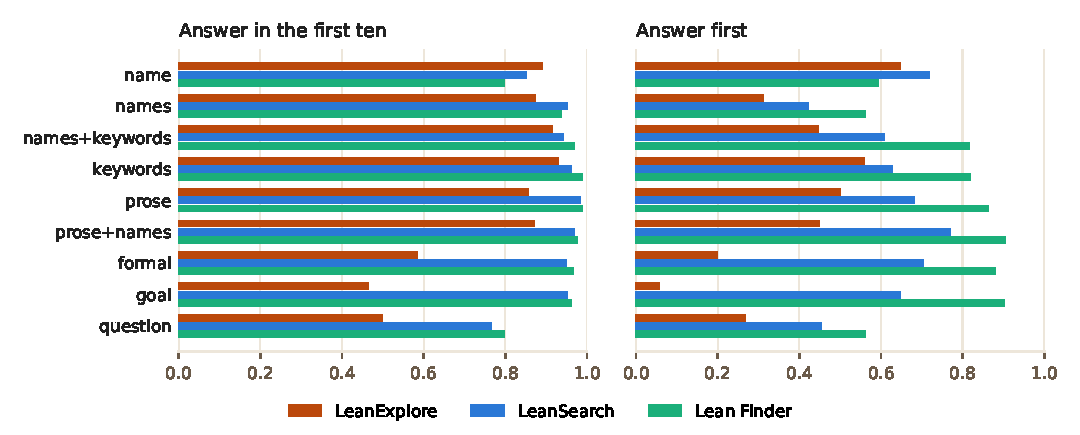
\includegraphics[width=\linewidth]{figures/forms.pdf}
\caption{Scores by form on the test split. \code{question} is the real
questions bucket. Table~\ref{tab:byform} adds BM25 and Loogle.}
\label{fig:forms}
\end{figure}

%=====================================================================
\section{Limitations and planned changes}
\label{sec:future}

\paragraph{No human review.} Queries, acceptance, and grades all come from
language models. We plan to have people review a sample and to report
agreement.

\paragraph{The pool covers four engines.} Answers that only a new engine
returns are unlabelled until they are graded (Section~\ref{sec:benchmark}).
The BM25 results above are in this position.

\paragraph{LeanExplore's descriptions.} The writer of a query sees
LeanExplore's natural-language description of the target, so written queries
may share wording with LeanExplore's index. The real questions bucket does not
have this bias.

\paragraph{Scope.} Version 1 covers Mathlib at one date, and every query has
an answer. Later versions will follow newer Mathlib snapshots and may add
other libraries and queries that have no answer.

\paragraph{Hosted engines change.} The scores above describe each service on
the dates given. We release the results we collected.

Each release of the benchmark will have a version number, and scores should be
reported with it.

%=====================================================================
\section{Conclusion}

\bench\ is a fixed set of 3,200 queries with graded answers for comparing
Lean declaration search engines. We will use it to measure changes to
LeanExplore, and we invite others to run their engines on it.

{\small
\bibliographystyle{plainnat}
\bibliography{references}
}

\clearpage
\appendix

\section{Scores by form}
\label{app:forms}

\begin{table}[H]
\centering\small
\caption{Success@10 on the test split by form, with Success@1 in brackets.
BM25 scores are lower bounds.}
\label{tab:byform}
\begin{tabular}{@{}lrrrrrr@{}}
\toprule
\thead{Form} & \thead{Queries} & \thead{Lean Finder} & \thead{LeanSearch} & \thead{LeanExplore} & \thead{BM25} & \thead{Loogle} \\
\midrule
\code{name} & 128 & 0.80 (0.59) & 0.85 (0.72) & 0.89 (0.65) & 0.88 (0.69) & 0.31 (0.31) \\
\rowrule
\code{names} & 64 & 0.94 (0.56) & 0.95 (0.42) & 0.88 (0.31) & 0.88 (0.14) & 0.11 (0.05) \\
\rowrule
\code{names+keywords} & 192 & 0.97 (0.82) & 0.94 (0.61) & 0.92 (0.45) & 0.72 (0.22) & 0.00 (0.00) \\
\rowrule
\code{keywords} & 256 & 0.99 (0.82) & 0.96 (0.63) & 0.93 (0.56) & 0.46 (0.18) & 0.00 (0.00) \\
\rowrule
\code{prose} & 384 & 0.99 (0.86) & 0.98 (0.68) & 0.86 (0.50) & 0.32 (0.12) & 0.00 (0.00) \\
\rowrule
\code{prose+names} & 256 & 0.98 (0.91) & 0.97 (0.77) & 0.87 (0.45) & 0.54 (0.14) & 0.00 (0.00) \\
\rowrule
\code{formal} & 384 & 0.97 (0.88) & 0.95 (0.70) & 0.59 (0.20) & 0.80 (0.34) & 0.16 (0.16) \\
\rowrule
\code{goal} & 256 & 0.96 (0.90) & 0.95 (0.65) & 0.46 (0.06) & 0.69 (0.23) & 0.00 (0.00) \\
\rowrule
\code{question} & 640 & 0.80 (0.56) & 0.77 (0.45) & 0.50 (0.27) & 0.24 (0.10) & 0.00 (0.00) \\
\bottomrule
\end{tabular}
\end{table}

\end{document}
